\chapter{Input files}
\label{sec:inputfiles}

\section{Mapping files}
\label{sec:mapping_files}

Mapping relates atomistic and coarse-grained representations of the system. It is organized as follows: for each molecule {\em type} a mapping file is created. When used as a command option, these files are combined in a list separated by a semicolon, e.~g. \progopt{---cg}~\texttt{"protein.xml;solvent.xml"}.

\begin{wrapfigure}{ht}{6cm}
  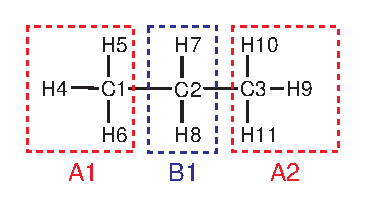
\includegraphics[width=6cm]{usage/fig/propane.eps}
  \caption{Atom labeling and mapping from an all-atom to a united atom representation of a propane molecule.
  \label{fig:propane_map}
}
\end{wrapfigure}

Each mapping file contains a {\em topology} of the coarse-grained molecule and a list of {\em maps}. Topology specifies coarse-grained beads and bonded interactions between them. Each coarse-grained bead has a name, type, a list of atoms which belong it, and a link to a map. A map is a \hyperref[sec:mapping_operator]{set of weights} $c_{Ii}$ for an atom $i$ belonging to the bead $I$. It is used to calculate the position of a coarse-grained bead from the positions of atoms which belong to it. Note that $c_{Ii}$ will be automatically re-normalized if their sum is not equal to 1, i.~e. in the case of a center-of-mass mapping one can simply specify atomic masses.
A complete reference for mapping file definitions can be found in sec.~\ref{sec:ref_mapping}.

As an example, we will describe here a mapping file of a united atom model of a propane molecule, chemical structure of which is shown in fig.~\ref{fig:intro:propane}. In this coarse-grained model two bead types (A,B) and three beads (A1, B1, A2) are defined, as shown in fig.~\ref{fig:propane_map}. We will use centers of mass of the beads as  coarse-grained coordinates.

Extracts from the \texttt{propane.xml} file of the tutorial are shown below. The \mapopt{name} tag indicates the molecule name in the coarse-grained topology. The \mapopt{ident} tag must match the name of the molecule in the atomistic representation. In the \mapopt{topology} section all beads are defined by specifying bead name (A1, B1, A2), type, and atoms belonging to this bead in the form \texttt{residue id:residue name:atom name}. For each bead a map has to be specified, which is defined later in \mapopt{maps} section. Note that bead \hyperlink{\mapref{topology.cg_beads.cg_bead.type}}{type} and \hyperlink{\mapref{maps.map}}{map} can be different, which might be useful in a situation when chemically different beads (A1, B1) are assigned to the same bead type. After defining all beads the bonded interactions of the coarse-grained molecule must be specified in the \hyperlink{\mapref{topology.cg_bonded}}{cg\_bonded} section. This is done by using the identifiers of the beads in the coarse-grained model. Finally, in the \hyperlink{\mapref{topology.cg_beads.cg_bead.mapping}}{mapping} section, the mapping coefficients are defined. This includes a weighting of the atoms in the topology section. In particular, the number of weights given should match the number of beads.

\section{Verification of a mapping}
\label{sec:mapping_verification}
Note that the \mapopt{ident} tag should match the molecule name in the reference system. A common mistake is that beads have wrong names. In this case, the \prog{csg_dump} tool can be used in order to identify the atoms which are read in from a topology file \texttt{.tpr}. This tool displays the atoms in the format \texttt{residue id:residue name:atom name}. For multicomponent systems, it might happen that molecules are not identified correctly. The workaround for this case is described in~\sect{sec:adv_topology}.

To compare coarse-grained and atomistic configurations one can use a standard visualization program, e.~g. \texttt{vmd}.  When comparing trajectories, one has to be careful, since \texttt{vmd} opens both a \texttt{.gro} and \texttt{.trr} file. The first frame is then the \texttt{.gro} file and the rest is taken from the \texttt{.trr} file. The coarse-grained trajectory contains only the frames of the  trajectory. Hence, the first frame of the atomistic run has to be removed using the \texttt{vmd} menu.


\begin{figure}
\centering
\framebox{
\lstinputlisting{functionality/propane.xml}
}
\caption{An extract from the mapping file \texttt{propane.xml} of a propane molecule. The complete file can be found in the \texttt{propane/single\_molecule} tutorial.}
\end{figure}

\section{Advanced topology handling}
\label{sec:adv_topology}
A topology is completely specified by a set of beads, their types, and a list of bonded interactions. \votca is able to read topologies in the \gromacs \texttt{.tpr} format. For example, one can create a coarse-grained topology based on the mapping file and atomistic \gromacs topology using \prog{csg_gmxtopol}.
\begin{verbatim}
  csg_gmxtopol --top topol.tpr --cg propane.xml --out out.top
\end{verbatim}


In some cases, however, one might want to use a .pdb file which does not contain all information about the atomistic topology. In this case, additional information can be supplied in the \xml mapping file.

A typical example is lack of a clear definition of molecules, which can be a problem for simulations with several molecules with multiple types. During coarse-graining, the molecule type is identified by a name tag as names must be clearly identified. To do this, it is possible to read a topology and then modify parts of it. The new \xml topology can be used with the \progopt{---tpr} option, as any other topology file.

For example, if information about a molecule is not present at all, one can create one from a \texttt{.pdb} file as follows
\begin{lstlisting}
<topology base="snapshot.pdb">
  <molecules>
    <clear/>
    <define name="mCP" first="1" nbeads="52" nmols="216"/>
  </molecules>
</topology>
\end{lstlisting}
where $<$clear/$>$ clears all information that was present before.

Old versions of \gromacs did not store molecule names. In order to use this feature, a recent \texttt{.tpr} file containing molecule names should always be provided. For old topologies, rerun \gromacs \progex{grompp} to update the old topology file.

If molecule information is already present in the parent topology but molecules are not named properly (as it is the case with old \gromacs \progopt{.tpr} files), one can rename them using
\begin{lstlisting}
 <topology base="topol.tpr">
   <molecules>
     <rename name="PPY3" range="1:125"/>
     <rename name="Cl" range="126:250"/>
   </molecules>
 </topology>
\end{lstlisting}
Here, the file \progopt{topol.tpr} is loaded first and all molecules are renamed afterwards.

\section{Trajectories}
\label{sec:trajectory}

A trajectory is a set of frames containing coordinates (velocities and forces) for the beads defined in the topology. \votca currently supports \texttt{.trr}, \texttt{.xtc}, \texttt{.pdb} and \texttt{.gro} trajectory formats.

Once the mapping file is created, it is easy to convert an atomistic to a coarse-grained trajectory using \prog{csg_map}
\begin{verbatim}
  csg_map --top topol.tpr --trj traj.trr --cg propane.xml --out cg.gro
\end{verbatim}

The program \prog{csg_map} also provides the option \progopt{---no-map}. In this case, no mapping is done and \prog{csg_map} works as a trajectory converter. In general, mapping can be enabled and disabled in most analysis tools, e.g. in \prog{csg_stat} or \prog{csg_fmatch}.

Note that the topology files can have a different contents as bonded interactions are not provided in all formats. In this case, mapping files can be used to define and relabel bonds.

Also note that the default setting concerning mapping varies individually between the programs. Some have a default setting that does mapping (such as \prog{csg_map}, use \progopt{---no-map} to disable mapping) and some have mapping disabled by default (e.g. \prog{csg_stat}, use \progopt{---cg} to enable mapping).

\section{Setting files}
\label{sec:setting_files}

\begin{figure}[h]
\centering
\begin{lstlisting}[frame=single]
<cg>
  <non-bonded> <!-- non-bonded interactions -->
    <name>A-A</name> <!-- name of the interaction -->
    <type1>A</type1> <!-- types involved in this interaction -->
    <type2>A</type2>
    <min>0</min>  <!-- dimension + grid spacing of tables-->
    <max>1.36</max>
    <step>0.01</step>
    <inverse>
      ... specific commands
    </inverse>

    ... specific section for inverse boltzmann, force matching etc.
  </non-bonded>
</cg>
\end{lstlisting}
\caption{Abstract of a \texttt{settings.xml} file. See sec. \ref{sec:preparing_the_run} for a full version.}
\end{figure}

A setting file is written in the format \texttt{.xml}. It consists of a general section displayed above, and a specific section depending on the program used for simulations. The setting displayed above is later extended in the sections on iterative boltzmann inversion (\prog{csg_inverse}), force matching (\prog{csg_fmatch}) or statistical analysis (\prog{csg_stat}).

Generally, \prog{csg_stat} is an analysis tool which can be used for computing radial distribution functions and analysing them. As an example, the command

\begin{verbatim}
  csg_stat --top topol.tpr --trj traj.xtc --options settings.xml
\end{verbatim}

computes the distributions of all interactions specified in \texttt{settings.xml} and writes all tabulated distributions as files \texttt{``interaction name''.dist.new}.

\section{Table formats}
\label{sec:table_formats}
Distribution functions, potentials and forces are returned as tables and saved in a file. Those tables generally have the format
\begin{verbatim}
  x y [error] flag
\end{verbatim}
where \texttt{x} is input quantity (e.g. radius $r$, angles $\theta$ or $\phi$), \texttt{y} is the computed quantity (e.g. a potential) and \texttt{[error]} is an optional error for \texttt{y}. The token \texttt{flag} can take the values \texttt{i}, \texttt{o} or \texttt{u}.
In the first case, \texttt{i} (\texttt{in range}) describes a value that lies within the data range, \texttt{o} (\texttt{out of range}) symbolises a value out of the data range and \texttt{u} stands for an \texttt{undefined} value.

The token \texttt{flag} will be important when extrapolating the table as described in sec. \ref{sec:post_processing}.

%\section{Data files}
%\label{sec:data_files}
%\begin{verbatim}
%  csg_partdist
%\end{verbatim}
%extra file formats etc. \todo